 \thispagestyle{gocconone}
\pagestyle{gocco}
\everymath{\color{gocco}}
\graphicspath{{../gocco/pic/}}
\blfootnote{$^1${\color[named]{gocco}Trung tâm Quy hoạch và Điều tra tài nguyên -- môi trường biển khu vực phía Nam.}}
\begingroup
\AddToShipoutPicture*{\put(0,616){\includegraphics[width=19.3cm]{../bannergocco}}}
\AddToShipoutPicture*{\put(77,520){\includegraphics[scale=1]{../tieude.pdf}}} 
\centering
\endgroup

\vspace*{190pt}
\begin{multicols}{2}
	Một trong những tiêu chuẩn rõ ràng và thực tế nhất để phân định thắng bại trong mỗi ván đấu là bắt được Tướng đối phương (chiếu bí hoặc khóa cho đối phương hết nước đi). Muốn thực hiện được điều này, các kỳ thủ cần sở hữu kỹ năng vận dụng các đòn phối hợp, tấn công, và dứt điểm một cách sắc bén, hiệu quả và chuẩn xác. Do đó, ``sát cuộc" hay còn gọi là ``sát pháp" chính là kỹ năng đầu tiên và cơ bản nhất mà mỗi người chơi cờ đều phải nắm bắt và vận dụng một cách thuần thục trong thực chiến. Đó cũng được xem là dạng cờ thế đơn giản mà mỗi nước đi đều phải đạt được độ chính xác tuyệt đối. 
	\vskip 0.1cm
	Trên thực tế cho thấy, có nhiều kỳ thủ chơi rất hay ở $2$ giai đoạn đầu của ván đấu: khai cuộc hợp lý, hài hòa và chặt chẽ; trung cuộc nhạy bén, tính toán sâu sắc, nhưng lại lộ ra những điểm yếu khi bắt đầu những thời điểm mang tính chất quyết định: không linh hoạt, ra đòn thiếu chuẩn xác, không ít trường hợp đã bỏ lỡ những cơ hội giành thắng lợi, thậm chí còn bị phản kích bất ngờ và thua ngược, bỏ phí đi bao nhiêu tâm huyết cũng như công sức từ đầu ván cờ 
	khi đã sắp đến cuối đoạn đường dẫn đến thắng lợi. 
	\vskip 0.1cm
	Để tránh lặp lại những tình huống kể trên trong tương lai, chẳng còn cách nào khác là mỗi kỳ thủ cần học tập, củng cố, trau dồi thường xuyên kỹ năng dứt điểm của mình. Việc này cũng cần phải có kế hoạch cụ thể và trình tự, từ cơ bản đến nâng cao, từ đơn giản đến phức tạp, từ ít quân đến nhiều quân, từng bước rèn luyện khả năng tính nhẩm, thành thục thứ tự và nắm vững điều kiện xảy ra sát cục.
	\vskip 0.1cm
	Dưới đây là một vài hình cờ sát cuộc  điển hình trong  để quý độc giả có thể vận dụng trong các ván đấu của mình:
	\begin{figure}[H]
		\vspace*{-5pt}
		\centering
		\captionsetup{labelformat= empty, justification=centering}
		\includegraphics[width= 0.4\textwidth]{1}
		\caption{\small\textit{\color{gocco}Hình $1$.}}
		\vspace*{-10pt}
	\end{figure}
	$1.$ Hình $1$, nếu nhìn qua bên Đỏ đang rơi vào trạng thái nguy cấp vì Đen sẵn sàng dùng song Xe và đơn Chốt bất cứ lúc nào, Đỏ còn Song Mã và đơn Xe, đơn Chốt nhưng thế công chưa thực sự rõ ràng. Tuy nhiên, Đỏ được quyền đi trước, liên tục tung ra những đòn sấm sét như sau:
	\vskip 0.1cm
	$\pmb{1)}$	C$4.1$ Tg$5-6$\quad  $\pmb{2)}$ X$1-4$ S$5.6$($*$)\quad $\pmb{3)}$ M$1.2$ Tg$6.1$ \quad$\pmb{4)}$ M$1/2$($**$) $(1- 0)$
	\vskip 0.1cm
	\textit{($*$): Với tầm nhìn và sự nhạy bén với sát cục cao, Đỏ đã nhận thấy có thể kết thúc ván đấu nên liên tục mạnh dạn phế Xe và Chốt, tạo điều kiện cho $2$ Mã sẵn sàng bắt tướng đối phương.
	\vskip 0.1cm
	($**$): Sau khi ép Tướng rời khỏi vị trí an toàn và Sĩ treo lên lộ $6$, Đỏ dùng song Mã chiếu bí, Đen vô phương chống đỡ.}
	\begin{figure}[H]
		\vspace*{-5pt}
		\centering
		\captionsetup{labelformat= empty, justification=centering}
		\includegraphics[width= 0.4\textwidth]{2}
		\caption{\small\textit{\color{gocco}Hình $2$.}}
		\vspace*{-10pt}
	\end{figure}
	$2.$ Hình $2$, đây là hình cờ trong giai đoạn trung cuộc, thoạt nhìn thì $2$ bên sẽ tiếp tục chiến đấu lâu dài vì quân lực trên bàn cờ còn còn nhiều và ngang nhau. Nhưng đỏ đã nhìn ra cách để kết thúc ván đấu như sau:  
	\vskip 0.1cm
	$\pmb{1)}$	X$8.9$ Tg$.1$\quad $\pmb{2)}$ P$1.2$ S$5.6$($*$)\quad $\pmb{3)}$ X$6.6$ X$5-4$\quad $\pmb{4)}$ P$5.3$($**$)
	\vskip 0.1cm
	\textit{($*$): Nhận thấy bên Đen có điểm yếu duy nhất là Tướng nằm ở vị trí không thực sự an toàn, Đỏ lập tức chớp thời cơ bằng $2$ nước chiếu liên tiếp, khiến cho cửu cung ở vào tình trạng báo động.
	\vskip 0.1cm
	($**$): Nước đổi Xe mang tính chiến lược, ép Đen phải bình Xe rời trục lộ quan trọng. Lúc này mặt Tướng rộng mở, đỏ tự do tấn Pháo tạo sát, Đen buộc phải đầu hàng.}
	\begin{figure}[H]
		\vspace*{-5pt}
		\centering
		\captionsetup{labelformat= empty, justification=centering}
		\includegraphics[width= 0.4\textwidth]{3}
		\caption{\small\textit{\color{gocco}Hình $3$.}}
		\vspace*{-10pt}
	\end{figure}
	$3.$ Hình $3$, Đen với sức mạnh $2$ Xe và $2$ Chốt áp sát cửu cung, đang phục rất nhiều đòn chiếu bí. Nhưng Đỏ được quyền đi trước đã nhìn thấy con đường để giành chiến thắng, Đỏ đã  ra đòn như sau: 
	\vskip 0.1cm
	$\pmb{1)}$	X$8-6$ Tg$4.1$($*$) \quad$\pmb{2)}$ M$2/4$ Tg$4.1$\quad $\pmb{3)}$ M$4.5$($**$) Tg$4/1$\quad $\pmb{4)}$ X$2.8$ Tg$4/1$\quad $\pmb{5)}$ P$4.7$ $(1-0)$.
	\vskip 0.1cm
	\textit{($*$): Nước phế xe đầy mạnh mẽ và uy lực, ép cho Tướng Đen phải ăn lên, qua đó tạo tiền đề dùng Mã chiếu để lấy nước tiên.
	\vskip 0.1cm
	($**$):  Sau $2$ nước đi, Đỏ đưa được Mã tới vị trí chiến lược, Đen chỉ có thể di chuyển Tướng một cách bị động, Đỏ nắm chắc \linebreak thắng lợi.}
	\vskip 0.1cm
	\textit{Chú thích: C: Chốt, X: Xe, M: Mã, P: Pháo, Tg: Tướng, S: Sĩ, T: Tượng.}
	\vskip 0.1cm
	\textbf{\color{gocco}Câu đố kỳ này:} Đỏ được quyền đi trước, sẽ chơi như thế nào để giành thắng lợi trong các hình cờ dưới đây:
	\begin{figure}[H]
		\vspace*{5pt}
		\centering
		\captionsetup{labelformat= empty, justification=centering}
		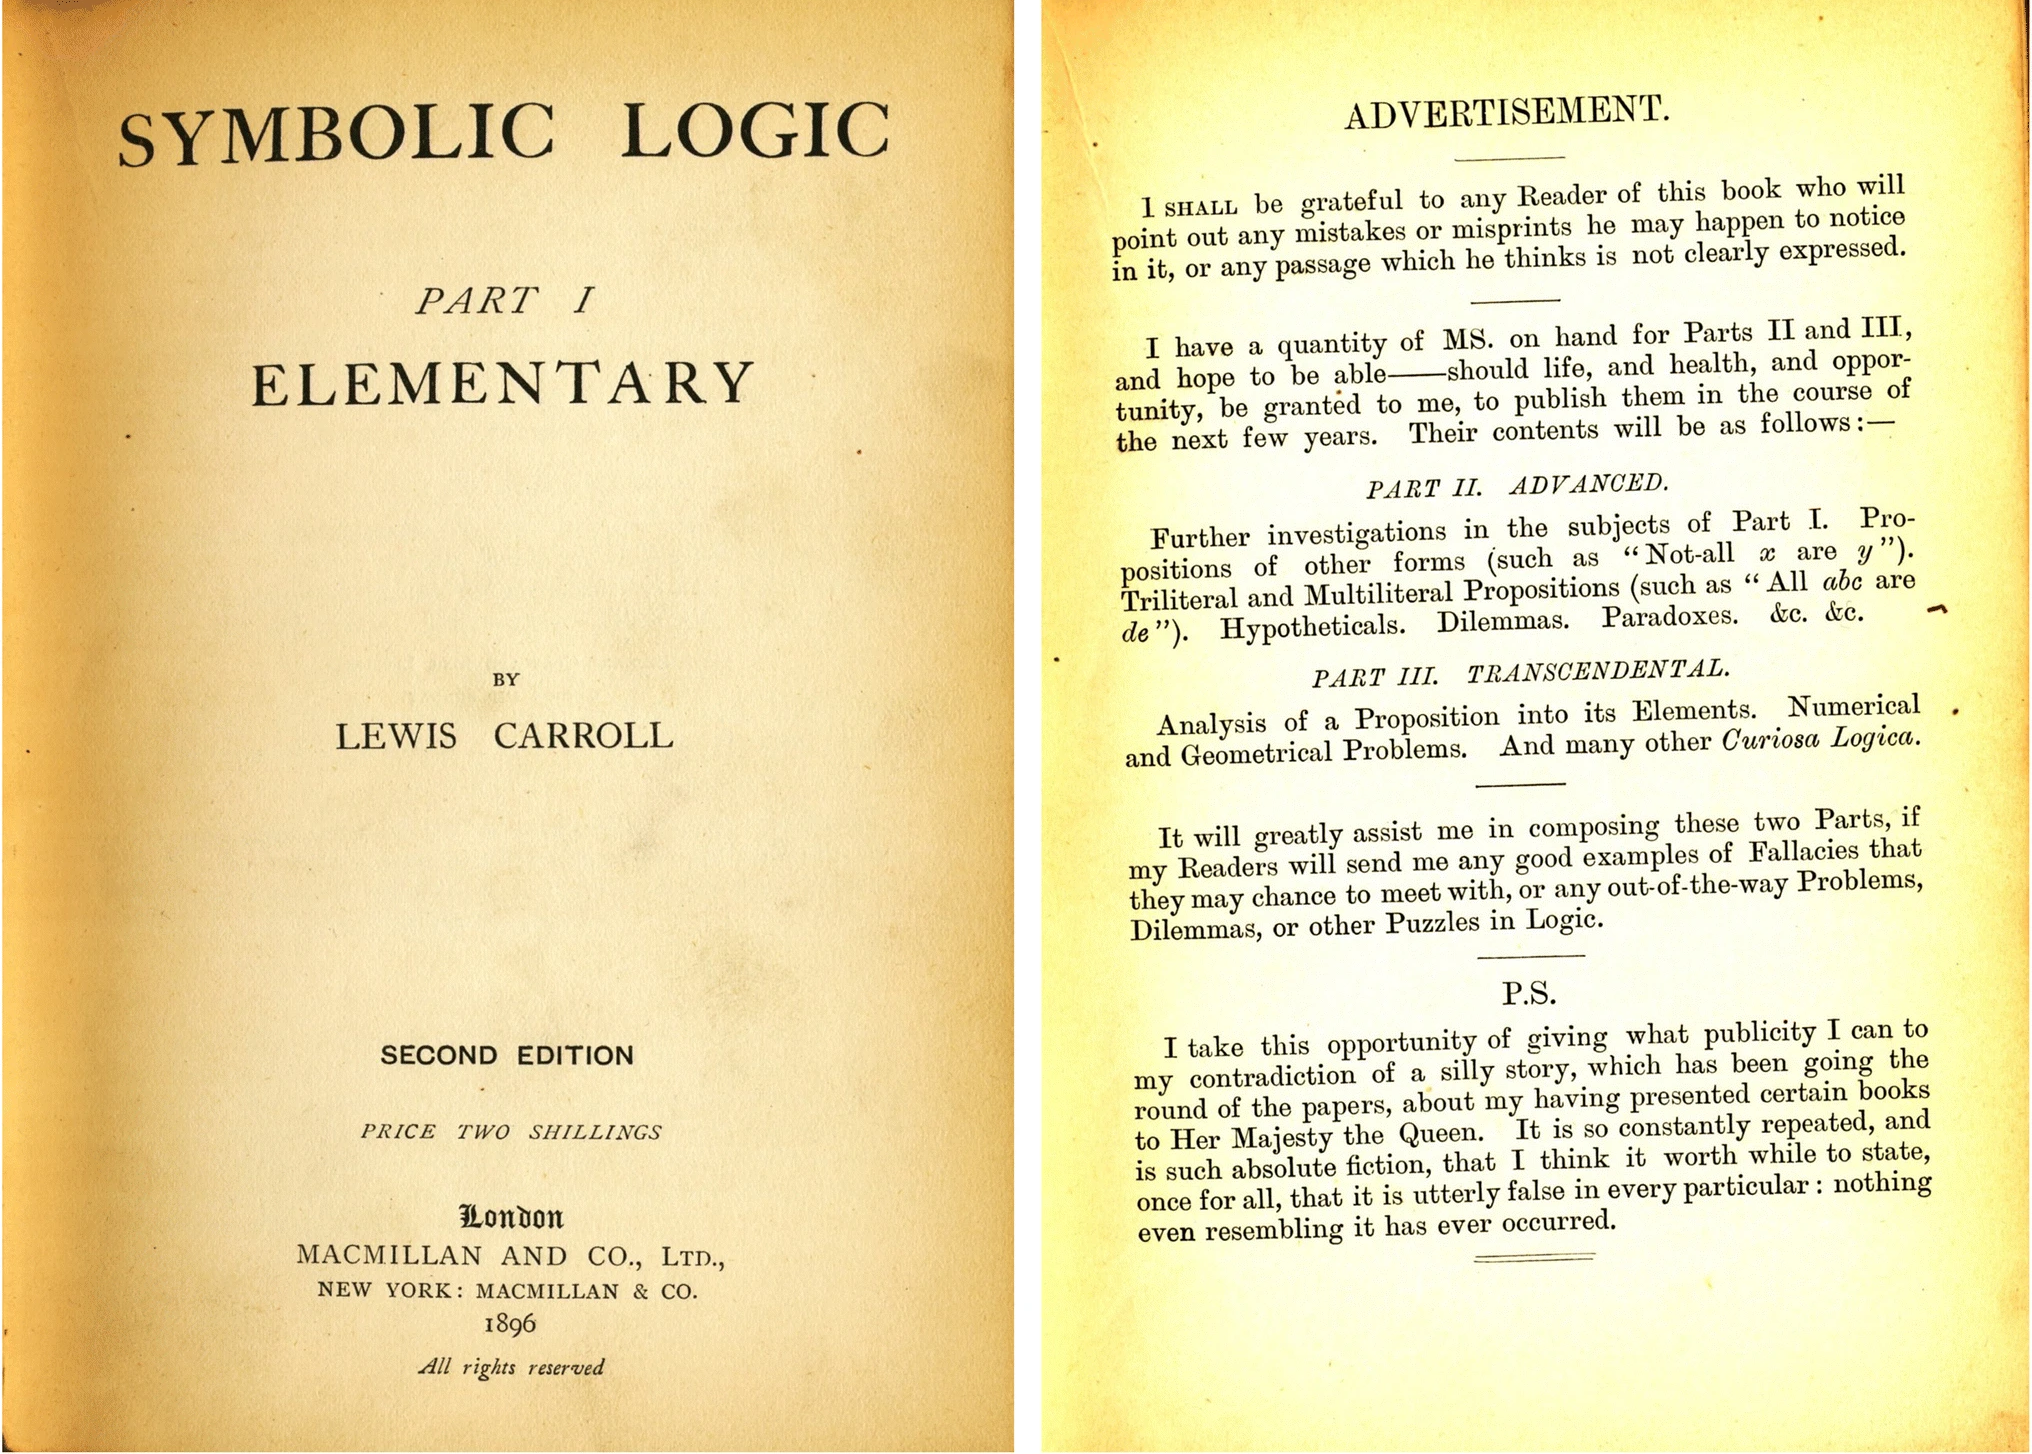
\includegraphics[width= 0.4\textwidth]{4}
		\caption{\small\textit{\color{gocco}Hình $4$.}}
		\vspace*{-10pt}
	\end{figure}
	\begin{figure}[H]
		\vspace*{5pt}
		\centering
		\captionsetup{labelformat= empty, justification=centering}
		\includegraphics[width= 0.4\textwidth]{5}
		\caption{\small\textit{\color{gocco}Hình $5$.}}
		\vspace*{-10pt}
	\end{figure}
\end{multicols}
\vspace*{-10pt}
\rule{1\linewidth}{0.1pt}
\begin{center}
	\vspace*{-5pt}
	\LARGE{\textbf{\color{gocco}LỜI GIẢI, ĐÁP ÁN}}
	\vspace*{-5pt}
\end{center}
\begin{multicols}{2}
	\textbf{\color{gocco}Cuộc họp kỳ lạ}
	\vskip 0.1cm
	Từ các tuyên bố ở lần thứ nhất suy ra không có hai người Trung thực nào ngồi cạnh nhau, và cũng không thể có $3$  người Nói dối ngồi cạnh nhau. Suy ra số người Trung thực không được quá nửa và không thể ít hơn một phần ba tổng số người tham gia. Vì thế số người Trung thực có thể là  $7$, $8$ hoặc $9$  người.
	\vskip 0.1cm
	Các tuyên bố của những người ở lại sau khi những người ``tẩy chay" bỏ đi chỉ có thể xảy ra trong hai trường hợp:
	\vskip 0.1cm
	$1)$	Tất cả họ đều là Trung thực (khi đó người cuối cùng rời đi cũng là người Trung thực).
	\vskip 0.1cm
	$2)$	Tất cả họ đều là Nói dối (khi đó người cuối cùng rời đi cũng là người Nói dối).
	\vskip 0.1cm
	Các tuyên bố của những người ``tẩy chay" cũng chỉ có thể xảy ra trong hai trường hợp:
	\vskip 0.1cm
	$1)$	Tất cả họ đều là Nói dối.
	\vskip 0.1cm
	$2)$	Cứ một người Nói dối lại có đúng  hai người Trung thực kế tiếp ngồi xếp quanh bàn. Khi đó số người Trung thực sẽ gấp đôi số người Nói dối trong số những người ``tẩy chay".
	\vskip 0.1cm
	Giả sử  chỉ toàn những người Trung thực ngồi lại chỗ cũ. Khi đó người cuối cùng rời bỏ cuộc họp cũng là Trung thực. Vì thế số người Trung thực trong số những người ``tẩy chay" phải bằng $2/3$  tổng số người ``tẩy chay". Tuy nhiên điều này mâu thuẫn do tổng số người Trung thực lúc đầu tiên không được quá nửa tổng số người tham gia (vì tất cả những người ngồi ở lại quanh chiếc bàn tròn cũ đều là người Trung thực).
	\vskip 0.1cm
	Vì thế chỉ toàn những người Nói dối ngồi lại chỗ cũ, và trong số những người rời bỏ, số người Trung thực phải gấp đôi số người Nói dối. Điều này chỉ xảy ra nếu số người Trung thực ban đầu là $8$  (do $7$  và $9$ là số lẻ). Do đó trong số những người ``tẩy chay" cuộc họp ban đầu, có đúng $8$ người Trung thực và $4$ người Nói dối. Vì vậy còn có $19-(8+4) = 7$  người vẫn ngồi lại ở vị trí cũ.
	\vskip 0.1cm
	\textbf{\color{gocco}Góc cờ}
	\vskip 0.1cm
	Hình $4$: $\pmb{1)}$	C$4.1$ Tg$5-4$\quad $\pmb{2)}$ P$3.5$ Tg$4.1$\quad $\pmb{3)}$ M$9.7$ Tg$4.1$\quad $\pmb{4)}$ M$3/4$ P$5/3$\quad $\pmb{5)}$ P$3/2$ $(1-0)$
	\vskip 0.1cm
	Hình $5$: $\pmb{1)}$	P$1.5$ P$7/2$\quad $\pmb{2)}$ C$6.1$ S$5/4$\quad $\pmb{3)}$ X$6.4$ Tg$5.4$\quad $\pmb{4)}$ X$3-6$ Tg$4-5$\quad $\pmb{5)}$ P$2-5$ $(1-0)$
\end{multicols}




